\section{Platform Design}
\label{sec:platform}

This section explains how we built our trading platform that can handle multiple participants at once. The platform has over 40 settings that researchers can adjust to control how the market works, how traders behave, and what experimental conditions to test. We provide all the parameter details with their mathematical symbols and default values in Appendix~\ref{app:parameters}.

\subsection{Market Structure}
\label{sec:market}

Our experimental market includes both human participants $\mathcal{N} = \{1, 2, \ldots, n\}$ and computer-controlled agents $\mathcal{A} = \{n+1, n+2, \ldots, m\}$. The human participants can be either informed traders $\mathcal{N}_I \subset \mathcal{N}$ or speculators. The computer agents include informed traders $\mathcal{A}_I \subset \mathcal{A}$ and noise traders $\mathcal{A}_N \subset \mathcal{A}$. Trading happens continuously over time from start $[0, \tau]$ where $\tau$ is how long the market stays open.

The platform keeps track of all buy orders $\mathbf{B}_t$ and sell orders $\mathbf{A}_t$ separately. Each order $o_i = (p_i, q_i, t_i)$ contains the price, quantity, and time when trader $i$ submitted it. When multiple orders have the same price, we combine their quantities. Orders execute immediately when the highest buy price meets or exceeds the lowest sell price:
\begin{equation}
\max(\mathbf{B}_t) \geq \min(\mathbf{A}_t)
\end{equation}

The platform keeps track of when each trader $i \in \mathcal{N} \cup \mathcal{A}$ places orders to ensure fair trading and accurate data recording.

\subsection{Parallel Market Creation}
\label{sec:sessions}

The platform can run multiple markets at the same time to collect data from different groups of participants. We call these parallel markets $\mathcal{M} = \{M_1, M_2, \ldots, M_j\}$, where each market $M_j$ works independently with its own group of participants $\mathcal{N}_j \subset \mathcal{N}$.

Participants join waiting pools $\mathcal{S}_s$ that have a fixed capacity $\nu_s = |\mathbf{g}|$, where $\mathbf{g} = [g_1, g_2, \ldots, g_{\nu_s}]$ is a list of trading goals we set up ahead of time. These goals tell participants what they should try to do: positive numbers mean they should buy that many shares, negative numbers mean they should sell that many shares, and zero means they should just try to make profit without specific targets. For example, if we set $\mathbf{g} = [100, -50, 0]$, we get one buyer (who should buy 100 shares), one seller (who should sell 50 shares), and one speculator.

We assign roles based on position in the pool: participant $k$ in pool $\mathcal{S}_s$ gets goal $g_k$ and role $r_k$ where:
\begin{equation}
r_k = \begin{cases}
\text{INFORMED} & \text{if } g_k \neq 0 \\
\text{SPECULATOR} & \text{if } g_k = 0
\end{cases}
\end{equation}

A new market starts when the waiting pool fills up completely ($|\mathcal{S}_s| = \nu_s$), which creates market $M_j$ with all the trading features ready to go. This wait-until-full approach lets us collect data from multiple independent markets running at the same time.

\subsection{Order Book Initialization}

Before participants join the market, the platform automatically places some initial orders to provide liquidity. This setup fills both the buy side $\mathbf{B}_0$ and sell side $\mathbf{A}_0$ of the order book with a predetermined number of orders.

For the initial buy orders, we randomly generate prices $p^{buy}_k$ from the range $[p_0 - \ell \cdot \sigma, p_0 - \sigma]$ for $k = 1, \ldots, \ell \times \omega$. For the initial sell orders, we generate prices $p^{sell}_k$ from the range $[p_0 + \sigma, p_0 + \ell \cdot \sigma]$. We then sort these prices so that:
\begin{align}
p^{buy}_1 \geq p^{buy}_2 \geq \cdots \geq p^{buy}_{\ell \times \omega} \\
p^{sell}_1 \leq p^{sell}_2 \leq \cdots \leq p^{sell}_{\ell \times \omega}
\end{align}

Each initial order has a quantity of $q = 1$, which creates balanced market depth on both sides around the starting price $p_0$ before human traders $\mathcal{N}$ start trading.

\subsection{Trader Endowments}

The market trades one asset (shares) for cash. We give traders different starting amounts of cash and shares depending on their type and the goals we assigned them in the session pools.

All human participants start with the same amount of cash and shares $(C_0, S_0)$, no matter what their assigned goals $g_i$ are. Their initial portfolio value is $W_0 = C_0 + S_0 \cdot p_0$. By giving everyone the same starting resources, we make sure that success depends on trading strategy, not on having more money or shares to begin with.

Computer agents get different starting resources based on what they're supposed to do. Noise traders get unlimited cash and shares $(C = \infty, S = \infty)$ so they can keep trading without running out of money. Informed computer traders get resources that match their goals: buying agents get $(2g_i \cdot p_0, 0)$ which gives them enough cash to complete their purchases, while selling agents get $(0, g_i)$ which gives them exactly the shares they need to sell, where $g_i$ is their target trading amount.

\subsection{Price Formation}

Market prices come from how participants trade with each other - there's no external price setting. The mid-price at time $t$ is the average of the best buy price and best sell price:
\begin{equation}
p_{mid,t} = \frac{\min(\mathbf{A}_t) + \max(\mathbf{B}_t)}{2}
\end{equation}

The bid-ask spread $s_t$ tells us how liquid the market is (smaller spreads mean more liquid):
\begin{equation}
s_t = \min(\mathbf{A}_t) - \max(\mathbf{B}_t)
\end{equation}

When the market closes, we need to deal with any orders that haven't executed yet so we can calculate final portfolio values and pay participants. The closure system makes sure everyone gets a definite payoff even if they have unfilled orders. For any remaining order with quantity $q$, we calculate closure prices as:
\begin{align}
p_{closure}^{buy} &= p_{mid,\tau} + q \cdot \Delta \cdot \kappa \\
p_{closure}^{sell} &= p_{mid,\tau} - q \cdot \Delta \cdot \kappa
\end{align}
where $\Delta$ is the default spread width and $\kappa$ is a penalty factor that makes larger orders more expensive. This pricing gives worse prices than normal market trading to discourage people from gaming the system by placing strategic orders right before the market closes.

\section{Trader Types}

\subsection{Human Traders}

Human traders make discrete choices about their orders. When trader $i$ wants to place an order at time $t$, they choose from available options $\mathcal{O}_i(t) = \{(p, q, \theta) : p \in \mathbb{R}^+, q \in \mathbb{N}, \theta \in \{-1, 1\}\}$ where $p$ is price, $q$ is quantity, and $\theta$ is whether it's a buy (+1) or sell (-1) order. The platform shows them pre-calculated price levels $P_t^{buy}, P_t^{sell}$ based on current best prices to help them make decisions quickly.

For informed traders $i \in \mathcal{N}_I$, we track how close they are to completing their goals by adding up their executed trades:
\begin{equation}
\pi_i(t) = \sum_{s=0}^{t} q_{i,s} \cdot \text{sign}(g_i)
\end{equation}
where $q_{i,s}$ is how much they traded at time $s$, and they complete their goal when $\pi_i(t) \geq |g_i|$.

The platform can optionally coordinate timing between human participants and computer traders. When this feature is turned on, human trading gets paused while computer traders are active, which prevents interactions that might mess up the experimental results. Researchers can choose whether to use this feature depending on their experimental design.

\subsection{Noise Traders}

Noise traders create background market activity using unlimited money and shares to keep the market liquid. Each time they act, they first might cancel an existing order (with probability $\epsilon$), then they place a new order.

Noise traders usually decide between buying and selling with probability $\zeta$ for buys. But they have a special rule: if there are no buy orders in the market, they only place buy orders; if there are no sell orders, they only place sell orders. This keeps both sides of the market active at all times.

When placing orders, noise traders choose between two types of trading:
\begin{align}
\mathbb{P}(\text{Passive}) &= \delta \\
\mathbb{P}(\text{Aggressive}) &= 1 - \delta
\end{align}

Passive orders add liquidity by placing orders at prices worse than the current best prices - these use prices $p = p_{best,t} \pm k \cdot \sigma$ where $k$ is a random distance from the best price, chosen from levels $\{1, 2, \ldots, \ell\}$. Aggressive orders consume liquidity by matching with existing orders at current market prices. Order sizes are chosen randomly up to a maximum of $q_{max}$ to make the trading look realistic.

\subsection{Informed Traders}

Informed traders use a conditional aggressive strategy that depends on how wide the spread is. They only trade when the current bid-ask spread $s_t$ is smaller than their edge parameter $\gamma$, where $\gamma$ is the maximum spread they're willing to pay. When $s_t \leq \gamma$, buying-oriented traders take the best sell price and selling-oriented traders take the best buy price. When $s_t > \gamma$, informed traders wait for the spread to narrow.

The platform can also let informed traders use passive strategies where they place limit orders at multiple price levels near the best prices, but the standard setup uses only the aggressive approach described above.

We set trading goals to match expected noise trader activity so the market stays balanced. The automatic goal calculation is:
\begin{equation}
g_i = \left\lfloor \frac{\beta}{1-\beta} \cdot \mathbb{E}[V_N] \right\rfloor
\end{equation}
where $\beta$ is how intense informed trading should be and $\mathbb{E}[V_N]$ is how much we expect noise traders to trade during the session. Informed traders stop trading when they complete their goals, which keeps the experiment controlled by preventing them from trading too much.

\subsection{Data Collection}

The platform records every trading action with precise timestamps, which lets researchers completely rebuild what happened in the market after the experiment. Instead of taking snapshots of the order book, we record each individual order placement, execution, and cancellation.

Each recorded event includes who the trader was, what the order details were, and exactly when it happened. From this sequence of events, researchers can rebuild everything about how the market evolved, including order book states, transaction histories, and participant portfolios at any moment during trading.

To rebuild the market, we replay the logged events in chronological order to reconstruct the market state $X_t = (\mathbf{B}_t, \mathbf{A}_t, p_{mid,t}, s_t, V_t)$ where $V_t$ is the total volume traded. We also track how each trader's cash and shares $(C_{i,t}, S_{i,t})$ changed over time for every trader $i \in \mathcal{N} \cup \mathcal{A}$. 

We calculate each trader's profit and loss using current market values:
\begin{equation}
\Pi_{i,t} = C_{i,t} + S_{i,t} \cdot p_{mid,t} - W_{i,0} \label{eq:pnl}
\end{equation}
where $W_{i,0}$ is what their portfolio was worth at the start.

\subsection{Platform Interface}
\label{sec:interface}

The platform gives participants a trading interface to make decisions in the electronic market. Understanding this interface is important because it determines how participants interact with the market systems we described above.

\subsubsection{Dashboard Layout}

The main trading interface has six information panels arranged in three columns, each serving different functions for trading, as shown in Figure~\ref{fig:dashboard}. The layout follows conventions from real financial trading platforms.

The header shows real-time information about each participant's portfolio, including their assigned role based on goal vector $\mathbf{g}$, their current profit and loss $\Pi_{i,t}$, how many shares they own with indicators showing changes, their cash $C_{i,t}$, and how many human traders are currently active versus how many we expected.

\begin{figure}[!htbp]
\centering
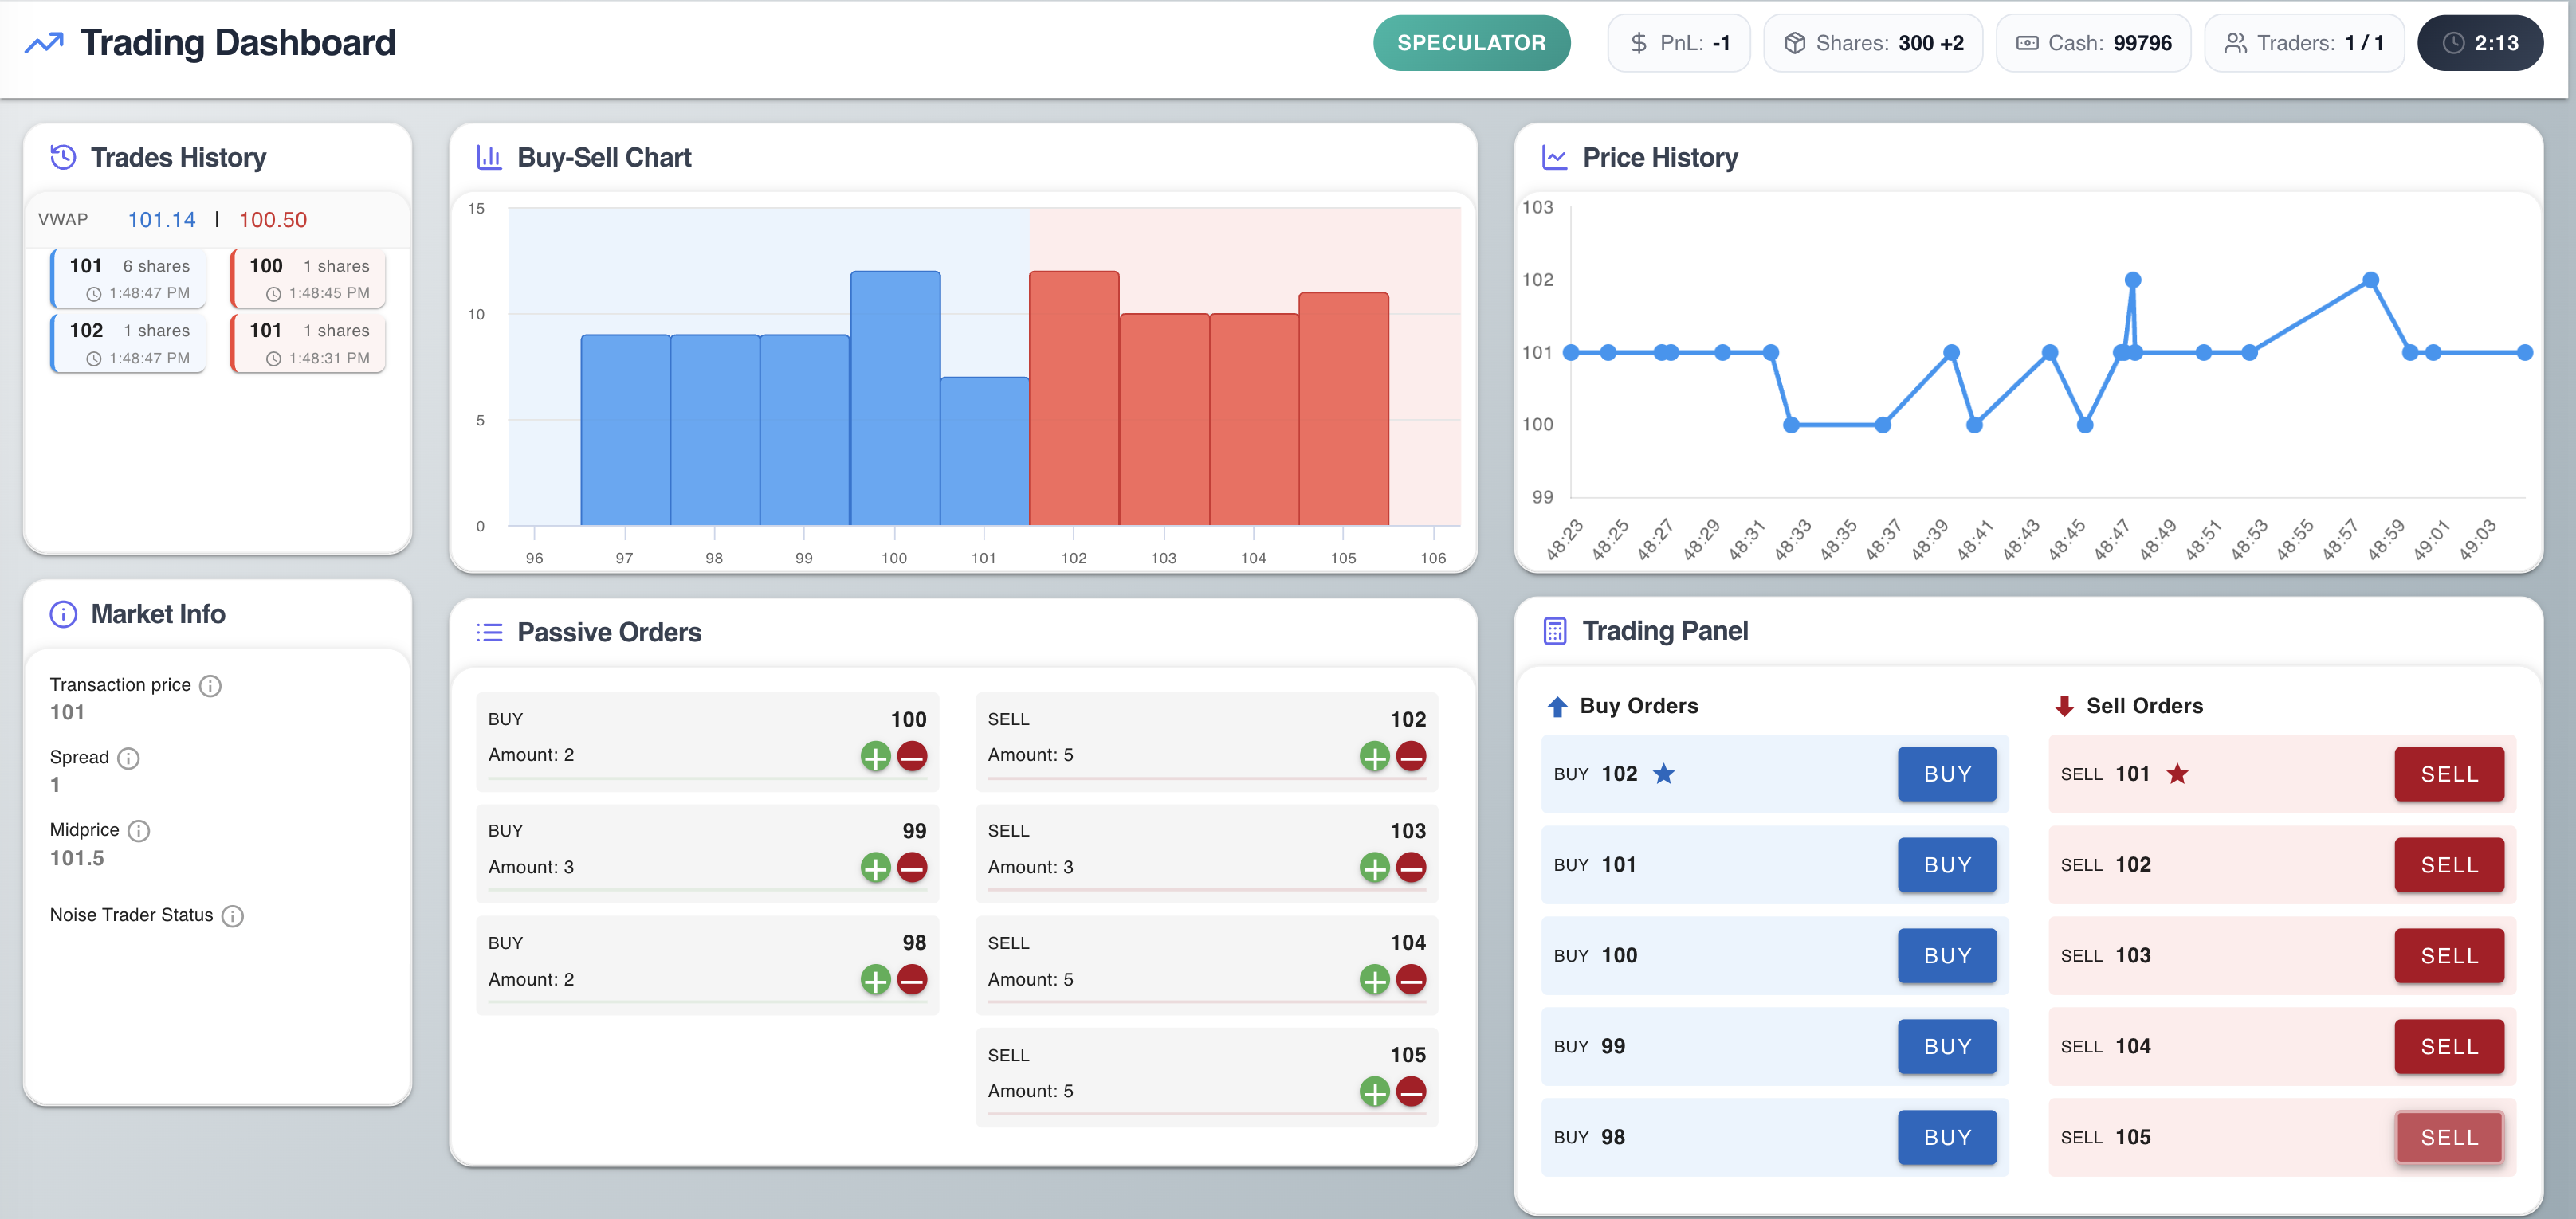
\includegraphics[width=0.95\textwidth]{figs/trading-dashboard.png}
\caption{Main Trading Interface. Six-panel layout showing trade history, market information, order book visualization, active orders, price history, and trading controls with portfolio status.}
\label{fig:dashboard}
\end{figure}

\subsubsection{Order Placement Interface}

The trading panel is in the right column and is where participants actually place their orders. It has two sections: one for buy orders and one for sell orders. Each section shows multiple price levels $P_t^{buy}$ and $P_t^{sell}$ with buttons that participants can click to execute trades.

The interface marks the best market prices with star icons. Depending on their assigned goals, some trading buttons are disabled: participants with $g_i > 0$ (buyers) cannot place sell orders, participants with $g_i < 0$ (sellers) cannot place buy orders, and all trading stops when they reach their goal $|\pi_i(t)| \geq |g_i|$ so the human trader can no longer place orders.

We calculate the price levels shown based on the current order book state $(\mathbf{B}_t, \mathbf{A}_t)$ and a step size parameter $\sigma$. The platform shows $\ell_{display}$ price levels above and below the current best prices. Order throttling parameters $\theta_{throttle}$ limit how fast participants can submit orders to prevent market manipulation.

When computer traders are active, pause notifications appear as banners on the screen, telling participants when human trading is temporarily disabled to prevent confusing interactions between human and computer trading strategies.

\subsubsection{Market Information Display}

The order book visualization occupies the center-left panel and presents bid-ask distribution as a dual-sided bar chart. Blue bars represent buy quantities at each price level, red bars show sell quantities. Background shading indicates the bid-ask spread region, with midpoint $p_{mid,t}$ marked.

The chart updates in real-time as orders are placed, executed, or cancelled, so participants can see how the market state changes. Through this visualization, participants can see how deep the market is and how liquid it is.

\subsubsection{Price History and Portfolio Tracking}

The price history chart (center-right panel) shows how transaction prices have changed over time using a line graph. Participants can see market trends and price momentum through this display.

The left column has two panels for managing portfolios. The active orders panel shows orders that haven't executed yet, and participants can add more orders at existing price levels or cancel orders using plus and minus buttons. The trade history panel shows completed transactions and calculates the volume-weighted average price (VWAP) for buy and sell trades:

\begin{align}
\text{VWAP}_{buy} &= \frac{\sum_{n} p_n \cdot q_n^{buy}}{\sum_{n} q_n^{buy}} \label{eq:vwap_buy}\\
\text{VWAP}_{sell} &= \frac{\sum_{n} p_n \cdot q_n^{sell}}{\sum_{n} q_n^{sell}} \label{eq:vwap_sell}
\end{align}

where $p_n$ and $q_n$ are the transaction prices and quantities for completed trades.

The interface provides tooltips to explain market information. Money amounts are shown in experimental currency units (Liras) with conversion rates to real compensation.

\subsubsection{Post-Market Summary Interface}

When the market closes, participants see a performance summary that shows statistics about the whole market and their individual trading performance, as shown in Figure~\ref{fig:summary}. The summary shows three types of information for analyzing the experiment and calculating participant compensation.

\begin{figure}[!htbp]
\centering
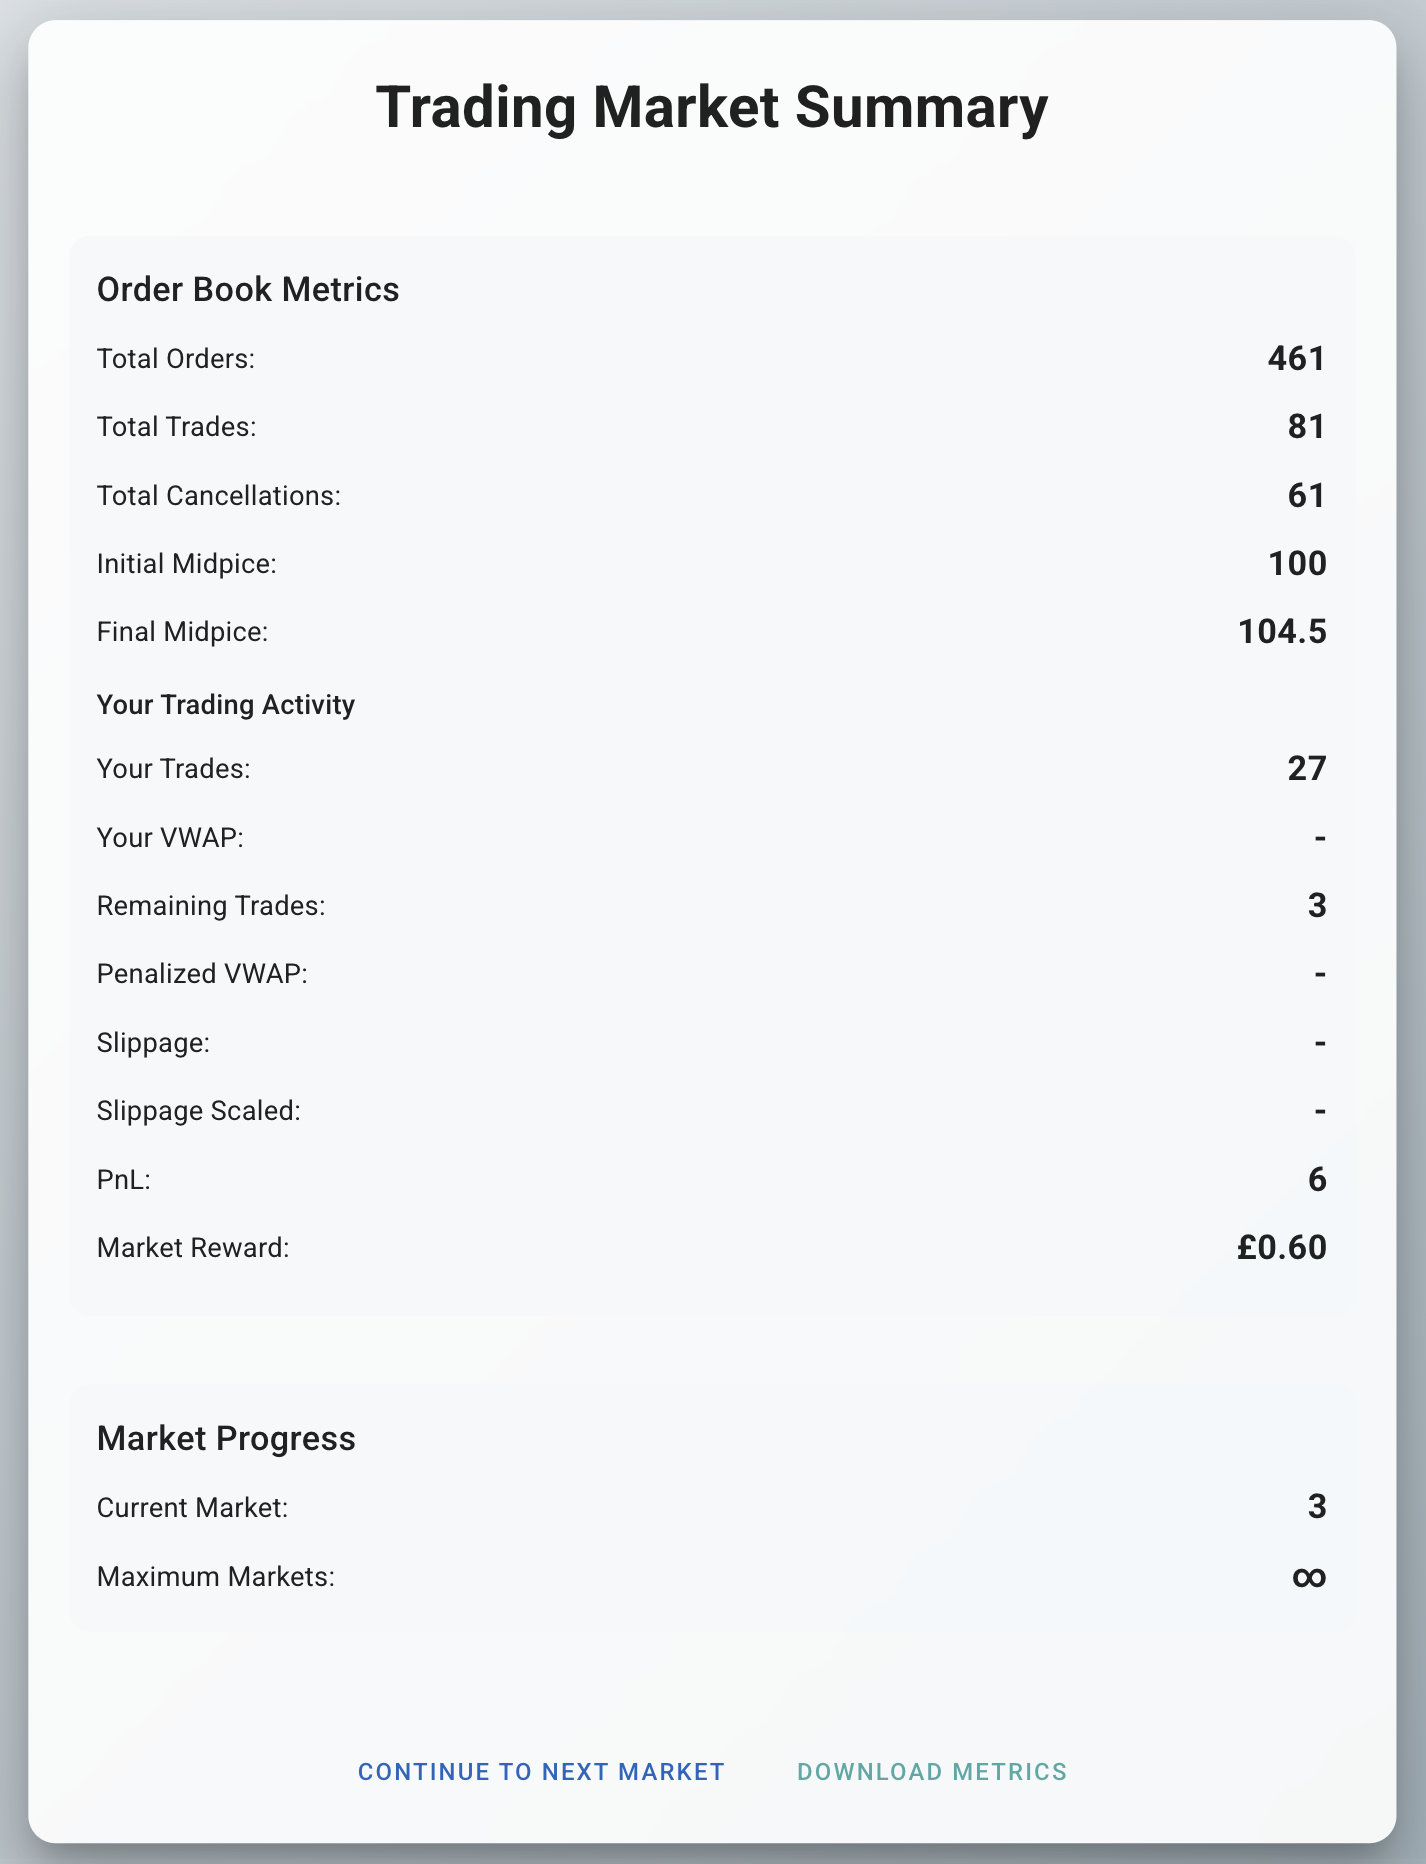
\includegraphics[width=0.7\textwidth]{figs/summary-page.png}
\caption{Post-Market Summary Interface. Trading metrics display including order book statistics, performance measures, and session progress with compensation calculations.}
\label{fig:summary}
\end{figure}

The Order Book Metrics section shows market-wide statistics that we reconstruct from the event log. Total orders, trades, and cancellations tell us how active the market was. The starting and ending midprices $p_{mid,0}$ and $p_{mid,\tau}$ show how price discovery worked during the trading session, which helps us assess market efficiency and price impact.

The Trading Activity section shows each trader's performance based on their assigned goals. The metrics include how many trades they completed, VWAP calculations using equations (\ref{eq:vwap_buy}) and (\ref{eq:vwap_sell}), and how many trades they still needed to complete their goals $g_i$. For participants who didn't complete their goals, the platform calculates penalized VWAP and slippage measures:

\begin{align}
\text{VWAP}_{penalized} &= \frac{\text{VWAP}_{actual} \cdot q_{executed} + p_{mid,\tau} \cdot \kappa \cdot q_{remaining}}{|g_i|} \label{eq:vwap_penalized}\\
\text{Slippage} &= \text{VWAP}_{penalized} - p_{mid,0} \label{eq:slippage}
\end{align}

where $q_{executed}$ is how many trades they completed, $q_{remaining} = |g_i| - q_{executed}$ is how many trades they still needed to complete their goal, and $\kappa$ is a penalty factor for not completing their target.

We calculate profit and loss using the mark-to-market method from equation (\ref{eq:pnl}), with portfolio values calculated when the market closes. We then convert trading performance into monetary compensation using performance-based scaling.

The Market Progress section keeps track of how participants advance through multiple experimental sessions. Market numbering and participation limits let researchers run repeated experiments while controlling for learning effects and participant fatigue.

\subsubsection{Administrative Interface}

The platform gives researchers an administrative interface for configuring settings, monitoring markets, and managing data, as shown in Figure~\ref{fig:admin}. The dashboard brings all control functions together in one place, letting researchers oversee and adjust parameters across multiple market sessions.

\begin{figure}[!htbp]
\centering
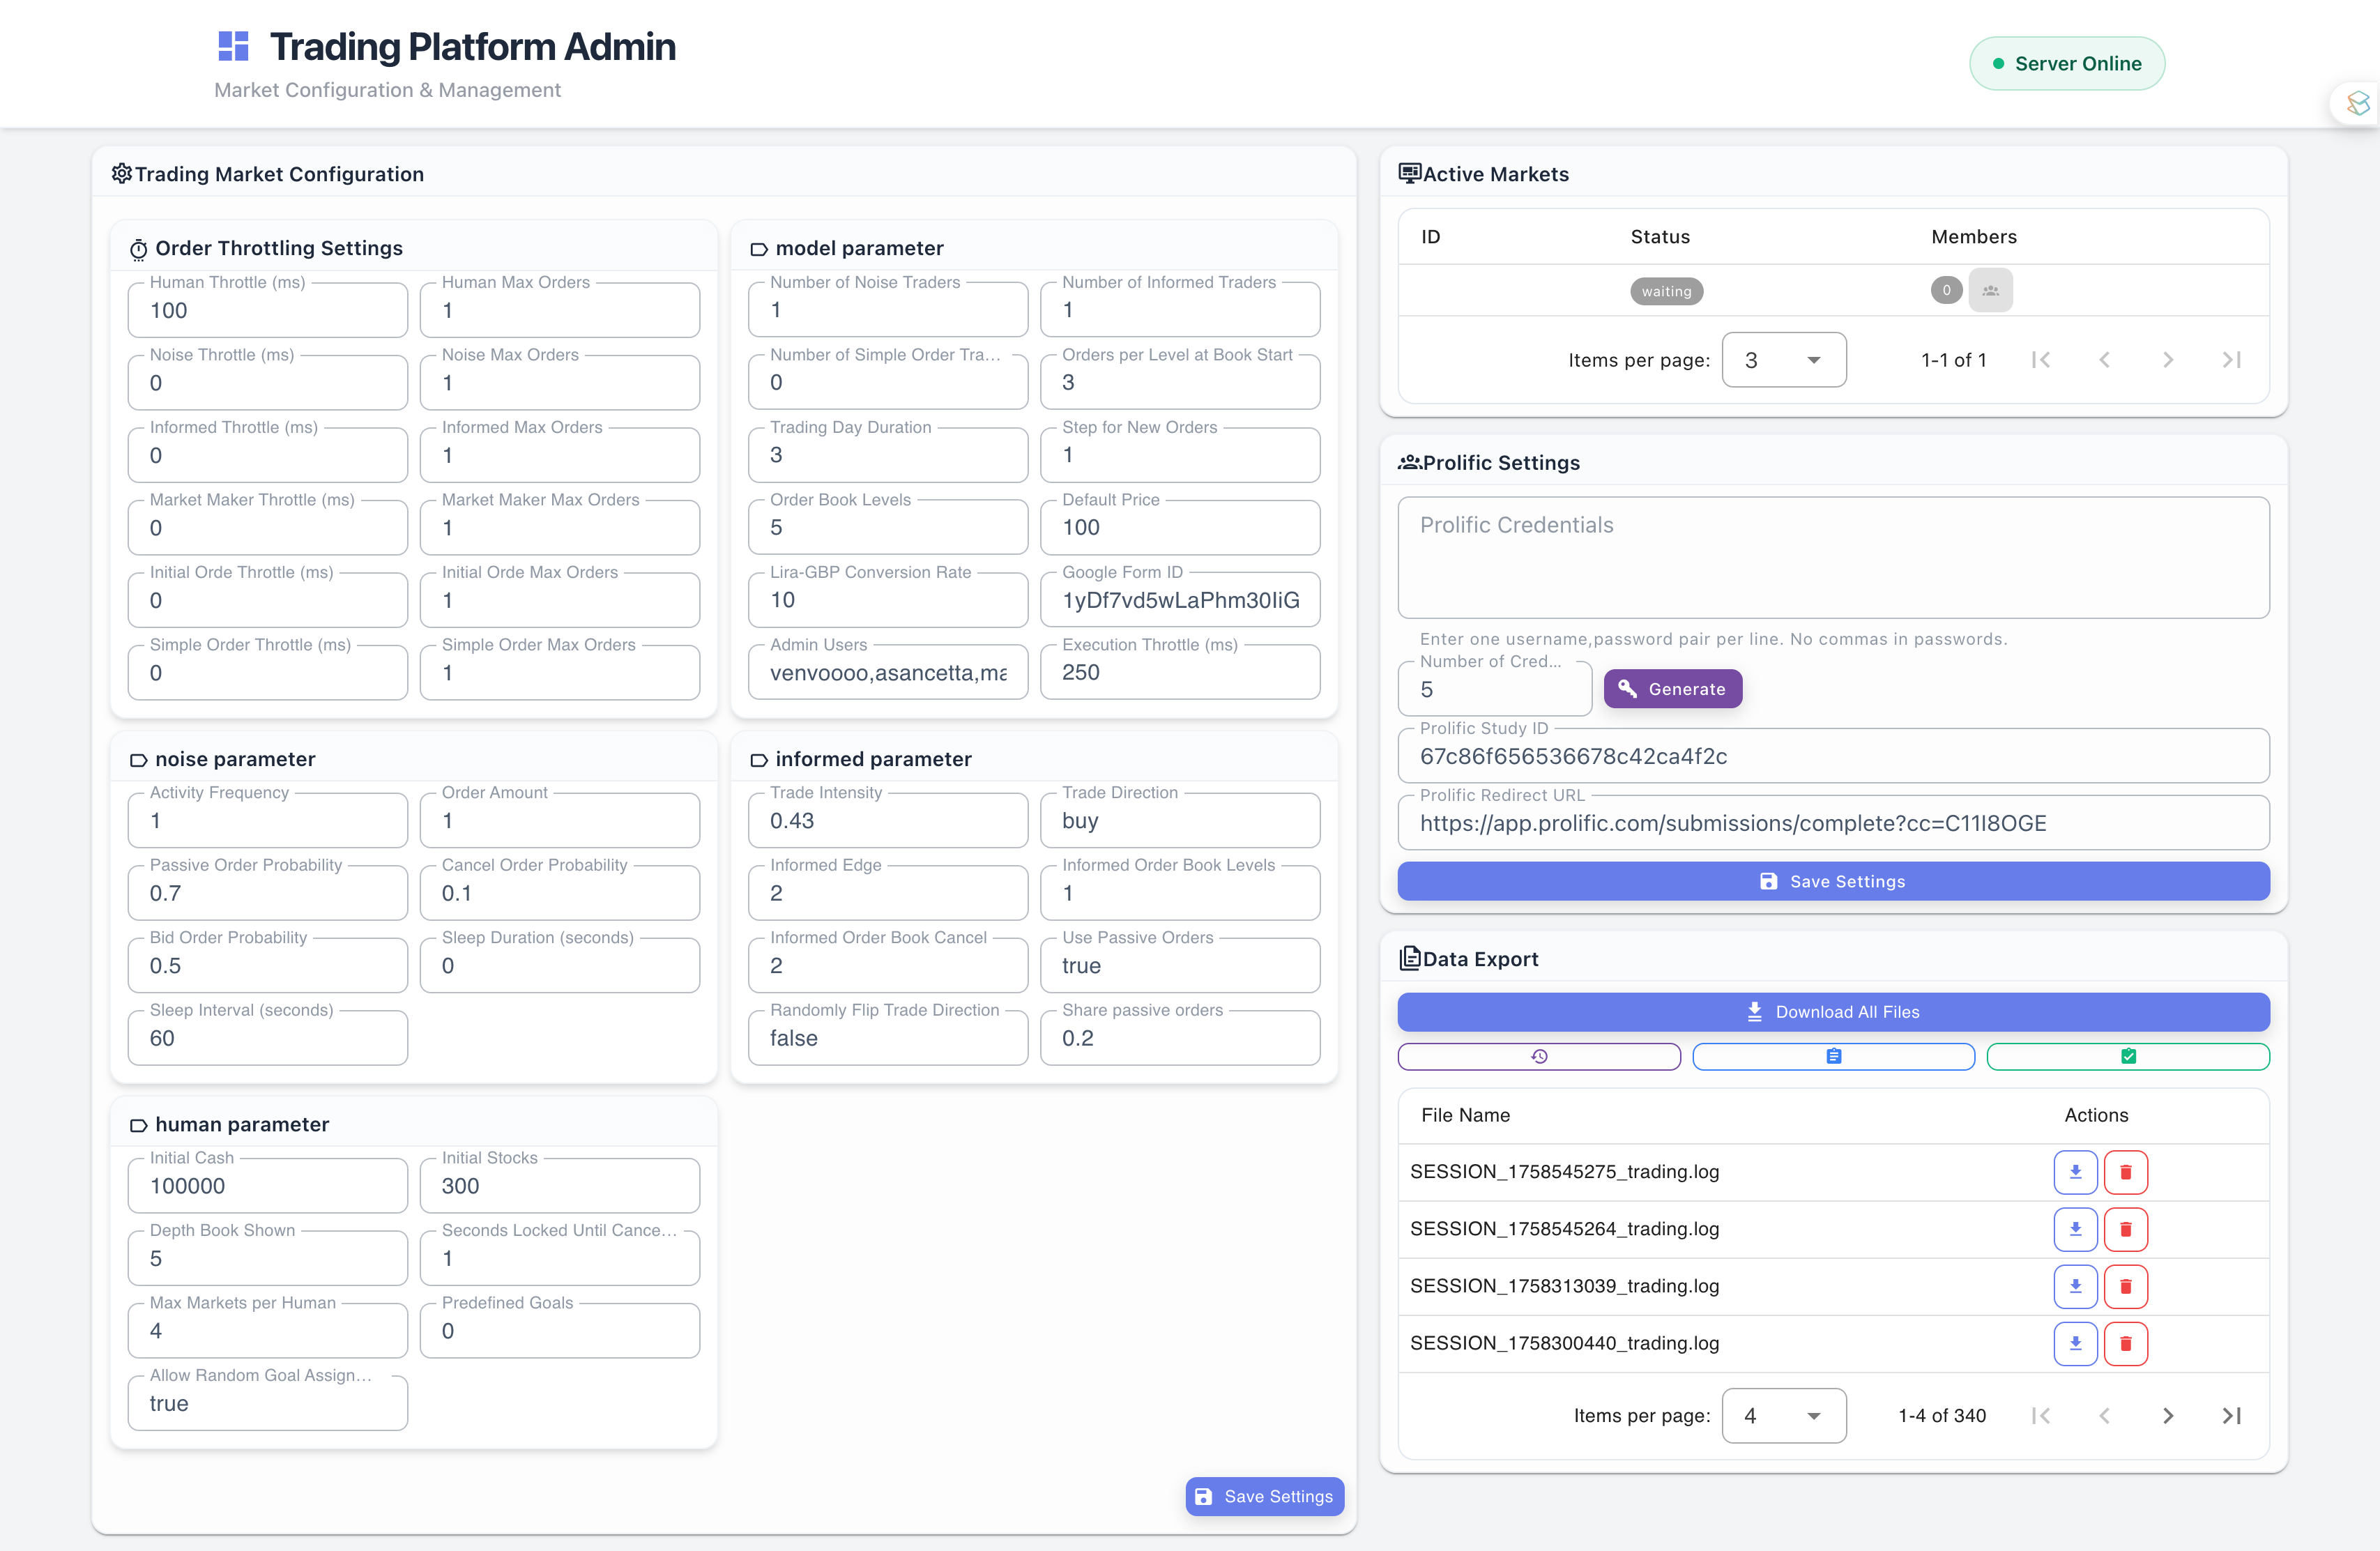
\includegraphics[width=0.95\textwidth]{figs/admin-page.png}
\caption{Administrative Interface Dashboard. Four main sections for market configuration with order throttling, active markets monitoring, Prolific integration, and data export.}
\label{fig:admin}
\end{figure}

The Trading Market Configuration panel organizes all the platform's settings into categories that match different trader types and market mechanisms. Parameters are grouped as model parameters (market structure), noise parameters (trader behavior), informed parameters (trader settings), and human parameters (participant endowments and interface settings). The interface highlights modified parameters $\theta_p \neq \theta_{p,default}$ to show which treatments differ from baseline conditions.

The Order Throttling section controls platform performance by limiting how fast different trader types can place orders. Each trader type gets throttling parameters $(\tau_{type}, \omega_{type})$ where $\tau_{type}$ is the milliseconds between orders and $\omega_{type}$ is the number of orders allowed per time window. This helps researchers balance realistic trading with computer system limitations.

The Active Markets Monitor shows the status of all parallel markets $\mathcal{M} = \{M_1, M_2, \ldots, M_j\}$ running at the same time. Each session entry shows how many participants have joined compared to how many are needed $|\mathcal{N}_j|/\nu_j$, the session status, and control buttons. The force-start feature lets researchers start markets even when they don't have enough participants, bypassing the normal wait-until-full rule when $|\mathcal{S}_s| < \nu_s$.

The Prolific Settings panel connects with research platforms by managing credentials and study settings. The platform creates and validates participant login information, manages study identifiers, and sets up redirect URLs for connecting with recruitment platforms like Prolific.

The Data Export section lets researchers download data for post-experiment analysis. The interface allows bulk data downloads, parameter history tracking, questionnaire response collection, and consent form management. File operations support data extraction while keeping data secure and protecting participant privacy.

\subsection{Trader Extensibility}
\label{sec:extensibility}

The platform lets researchers add new types of traders that work with all the market mechanisms we described above. This flexibility allows testing new behavioral models within controlled experimental environments.

\subsubsection{Basic Trader Setting}

All trader types are built on a common foundation that provides basic market interaction abilities. The platform automatically handles portfolio management $(C_{i,t}, S_{i,t})$, placing and canceling orders, communicating with the trading system, and tracking performance.

The platform uses standard communication methods. Each trader gets market updates including order book changes, trading session signals, market closure notifications, and transaction confirmations. The foundation provides standard behaviors that researchers can customize for specific trader types.

Order management follows the same procedures for all traders, including throttling limits, inventory updates, and platform communication. This makes sure all trader types operate under identical constraints and we collect consistent data.

The platform includes \texttt{SimpleOrderTrader} as an example that shows how to create custom trader types. This trader executes predetermined order sequences, giving researchers a concrete example of how to extend the basic trader framework.

\subsubsection{Shared Trading Environment}

All trader types have the same market access and face the same constraints. Each trader $i$ keeps track of their portfolio $(C_{i,t}, S_{i,t})$ and gets identical market information including the current order book state $(\mathbf{B}_t, \mathbf{A}_t)$, midpoint $p_{mid,t}$, and transaction history. The platform applies order throttling $\theta_{throttle}$ equally to all trader types to keep the experiment fair.

New trader types get the same information stream as existing traders: order executions, book updates, and timing signals. Custom trader types work with the parallel market creation and timing coordination systems, allowing studies where new behavioral models interact with human participants. Data collection works identically for custom traders, creating event logs that integrate with our reconstruction procedures to contribute to complete market state reconstruction $X_t = (\mathbf{B}_t, \mathbf{A}_t, p_{mid,t}, s_t, V_t)$.

\subsubsection{Behavioral Design Space}

Researchers can create traders with behaviors that cover the full range of existing trader types. Trading frequency can range from the continuous activity of noise traders to the discrete decisions of human traders. Order placement can follow fixed rules like informed traders or random patterns like noise traders.

Custom traders can be flexible with goal assignments - they can receive specific objectives $g_i$ from the session pool system or operate without goals like noise traders. Starting resources can follow any of the established patterns: uniform $(C_0, S_0)$, unlimited $(C = \infty, S = \infty)$, or goal-matched allocations.

\subsubsection{Example: Spread-Narrowing Market Maker}

Here's an example of a custom trader that provides liquidity by placing orders within the current bid-ask spread to make the market tighter. This trader watches the current best bid $p_{bid,t} = \max(\mathbf{B}_t)$ and best ask $p_{ask,t} = \min(\mathbf{A}_t)$, then places orders at better prices within the spread.

The trader's order placement strategy follows:
\begin{align}
p_{new\_bid} &= p_{mid,t} - \nu \cdot \frac{s_t}{2} \\
p_{new\_ask} &= p_{mid,t} + \nu \cdot \frac{s_t}{2}
\end{align}
where $\nu \in (0,1)$ is the spread improvement factor, $s_t = p_{ask,t} - p_{bid,t}$ is the current bid-ask spread, and $p_{mid,t}$ is the current midpoint.

This trader operates with unlimited money and shares $(C = \infty, S = \infty)$ to avoid budget constraints and continuously places limit orders at the improved prices with unit quantities. When orders execute, the trader immediately places new orders to maintain market presence. The trader cancels existing orders when market conditions change, keeping orders competitive.

Trader types like this enable studies of liquidity provision effects where researchers can examine how spread-narrowing behavior affects market quality measures including bid-ask spreads $s_t$, market depth, and price discovery efficiency.